\chapter{Results}
\label{chap:results}

\section{Validation}
\label{sec:validation}
Before we try to bring about new results, we should verify our method. For validation, we decided to replicate some results of Sychrovsky~\cite{Sychrovsky2020} for SCHW+BW and compare some of our basin maps for SCHW+BW with the Poincar\'e section from Polcar, Sukova and Semerak~\cite{Polcar2019}.

Our first validation case was Figure 4.3 in Sychrovsky~\cite{Sychrovsky2020}. 

\begin{figure}[H]
    \centering
    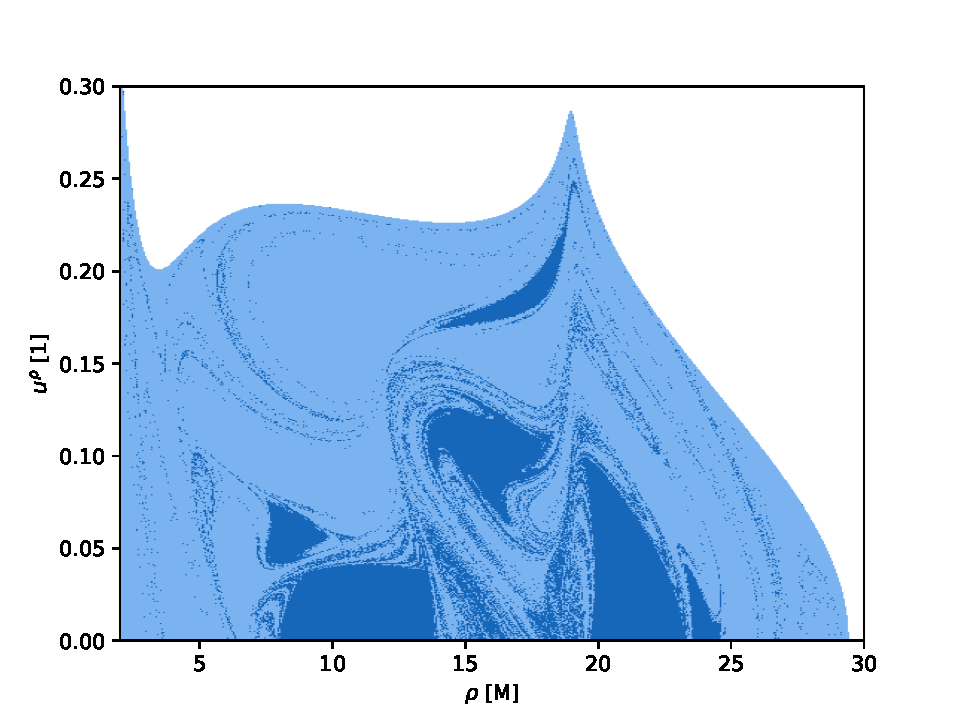
\includegraphics[width=0.9\linewidth]{img/basin_map_sch_bw_500_1.0_3.75_0.955_20.0_0.5_0.2_0_x86.pdf}
    \caption{Basin map (SCHW+BW) computed on a $500\times 500$ grid of initial conditions, $l=3.75M$, $\epsilon=0.955$, $b=20M$, $\mathcal{M}=0.5M$, $z=0.2$ (x86). \basinLegend}
    \label{fig:basin-map-500-l3p75-e0p955-b20-M0p5-z0p2-x86}
\end{figure}

\begin{figure}[H]
    \centering
    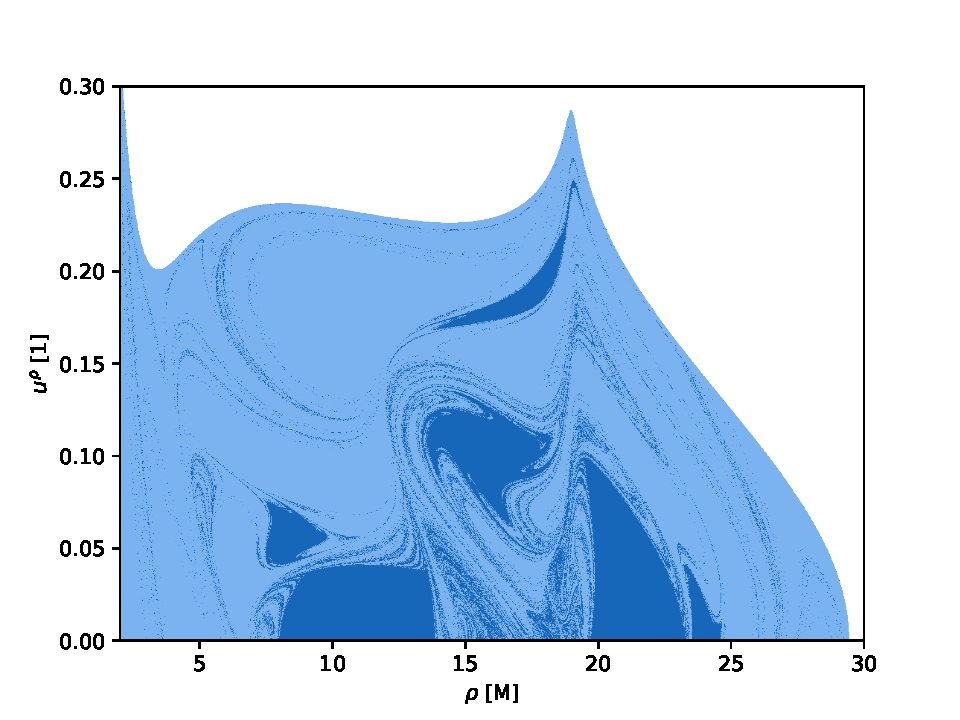
\includegraphics[width=0.9\linewidth]{img/basin_map_sch_bw_1000_1.0_3.75_0.955_20.0_0.5_0.2_0.pdf}
    \caption{Basin map (SCHW+BW) computed on a $1000\times 1000$ grid of initial conditions, $l=3.75M$, $\epsilon=0.955$, $b=20M$, $\mathcal{M}=0.5M$, $z=0.2$. \basinLegend}
    \label{fig:basin-map-1000-l3p75-e0p955-b20-M0p5-z0p2}
\end{figure}

Our basin map visually corresponds to Figure 4.3 in Sychrovsky~\cite{Sychrovsky2020} with $\lambda_{\text{stop}} = 0.02$. This correspondence can be explained by the fact that in our implementation, the stopping criterion is based on the exceeded relative tolerance for the conserved quantities. Therefore, the particle can get as close to the singularity as allowed by the tolerance.

The next validation case was Figure 5.5 in Sychrovsky~\cite{Sychrovsky2020} and the corresponding calculated fractal dimension.

\begin{figure}[H]
    \centering
    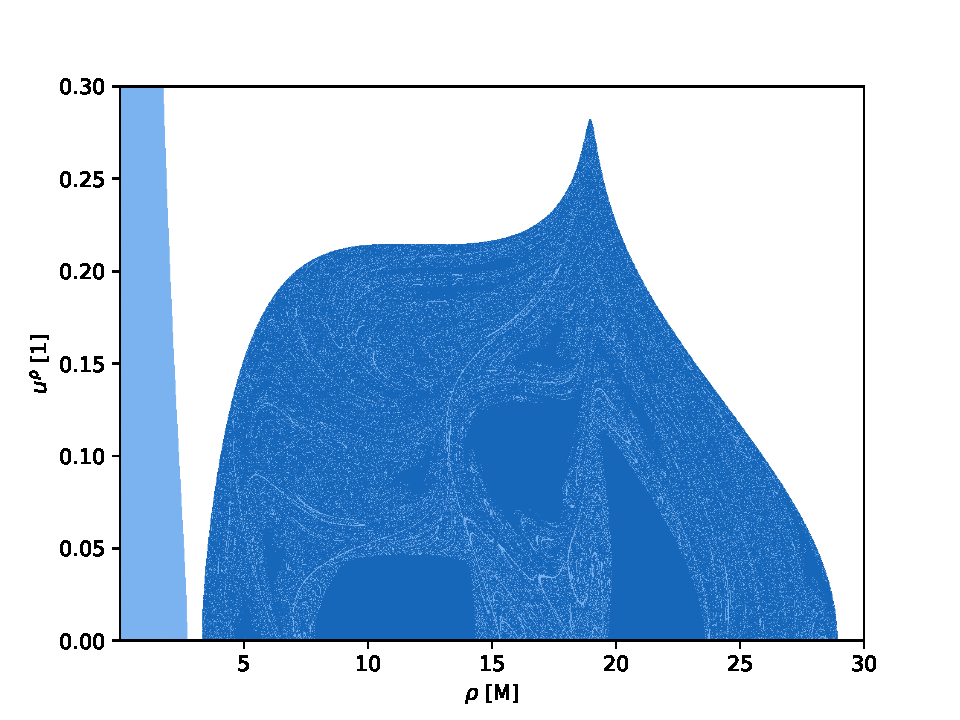
\includegraphics[width=0.82\linewidth]{img/basin_map_sch_bw_1000_1.0_3.943_0.955_20.0_0.5_0.2_0_whole_accessible_region.pdf}
    \caption{Basin map (SCHW+BW) of the whole accessible region; computed on a $1000\times 1000$ grid of initial conditions, $l=3.943M$, $\epsilon=0.955$, $b=20M$, $\mathcal{M}=0.5M$, $z=0.2$. \basinLegend}
    \label{fig:basin-schw-bw-1000-l3p943-e0p955-b20-M0p5-z0p2-whole}
\end{figure}

\begin{figure}[H]
    \centering
    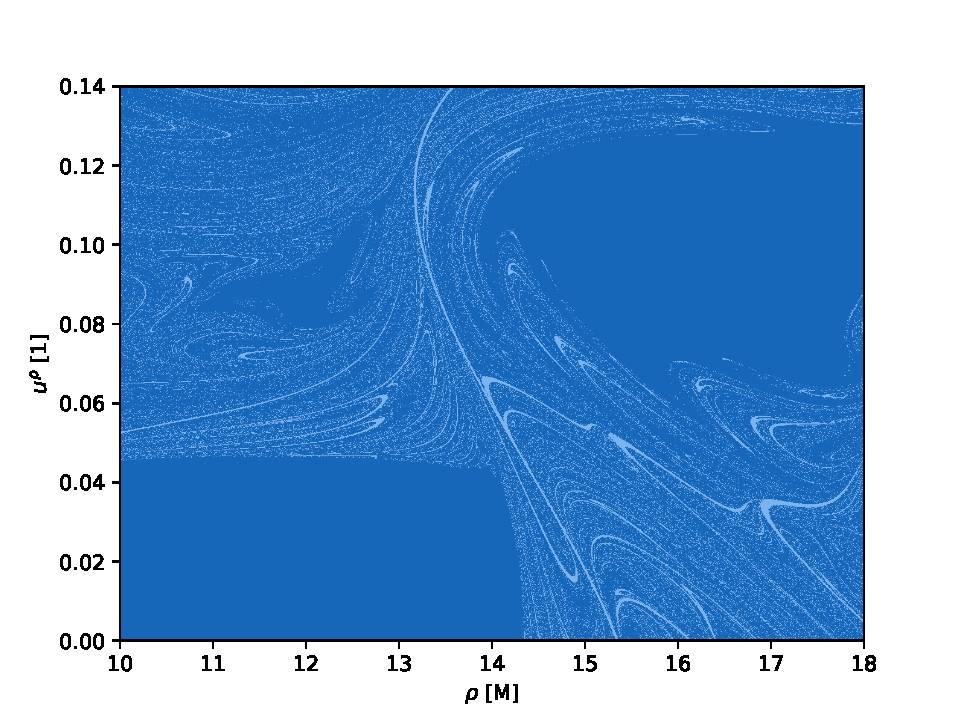
\includegraphics[width=0.82\linewidth]{img/basin_map_sch_bw_1000_1.0_3.943_0.955_20.0_0.5_0.2_0.pdf}
    \caption{Basin map (SCHW+BW) computed on a $1000\times 1000$ grid of initial conditions, $l=3.943M$, $\epsilon=0.955$, $b=20M$, $\mathcal{M}=0.5M$, $z=0.2$. \basinLegend}
    \label{fig:basin-schw-bw-1000-l3p943-e0p955-b20-M0p5-z0p2}
\end{figure}

\begin{figure}[H]
    \centering
    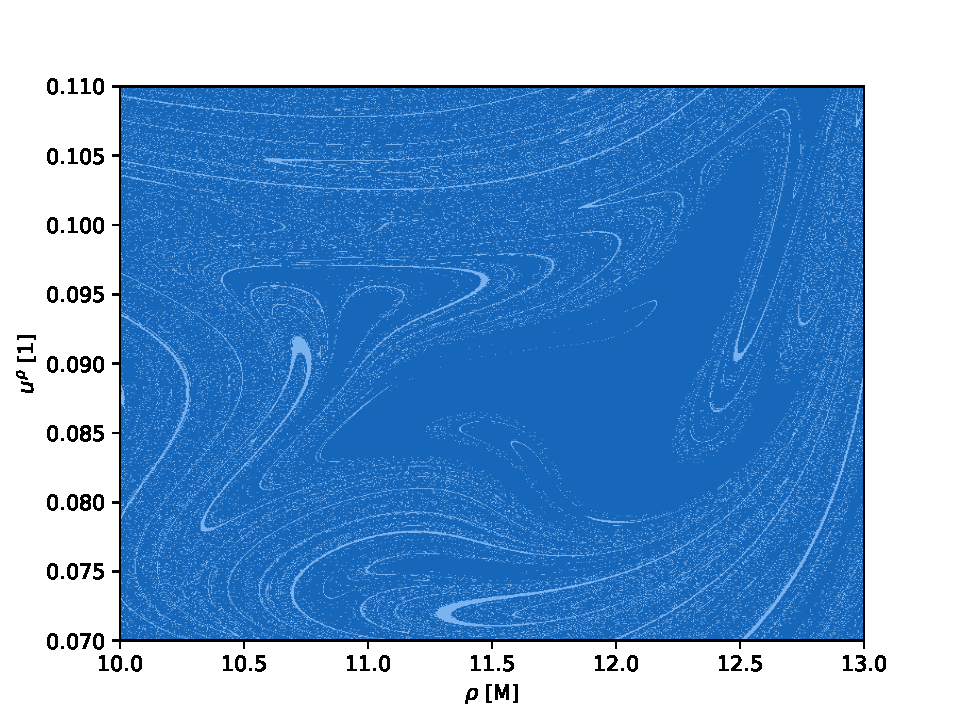
\includegraphics[width=0.82\linewidth]{img/basin_map_sch_bw_700_1.0_3.943_0.955_20.0_0.5_0.2_0.pdf}
    \caption{Basin map (SCHW+BW) computed on a $700\times 700$ grid of initial conditions, $l=3.943M$, $\epsilon=0.955$, $b=20M$, $\mathcal{M}=0.5M$, $z=0.2$. \basinLegend}
    \label{fig:basin-schw-bw-700-l3p943-e0p955-b20-M0p5-z0p2}
\end{figure}

\begin{figure}[H]
    \centering
    
\includegraphics[width=0.82\linewidth]{img/basin_map_sch_bw_500_1.0_3.943_0.955_20.0_0.5_0.2_0.pdf}
    \caption{Basin map (SCHW+BW) computed on a $500\times 500$ grid of initial conditions, $l=3.943M$, $\epsilon=0.955$, $b=20M$, $\mathcal{M}=0.5M$, $z=0.2$. \basinLegend}
    \label{fig:basin-schw-bw-500-l3p943-e0p955-b20-M0p5-z0p2}
\end{figure}

There are various reasons why our result may not fully correspond to the result of Sychrovsky~\cite{Sychrovsky2020}. In this case, the accessible region is divided into two parts. Hence, what we see in our zoomed basins are either eternal orbits or collisions with the disk, but no falls into the black hole. As mentioned by Sychrovsky, as $\lambda_{\text{stop}}$ increases, the basin of eternal orbits grows because the particles are allowed to move closer to the ring~\cite{Sychrovsky2020}. Since, as we found out, our implementation corresponds to the higher values of $\lambda_{\text{stop}}$ in the implementation in Sychrovsky~\cite{Sychrovsky2020}, therefore our basin has a richer basin $O$. However, other factors could also play a role, such as the fact that we used different codebases to create the basin. As mentioned earlier our solver was written for long double. On Apple silicon ARM64 with Apple Clang 17, long double has the same numerical precision as double. On the x86\_64 Linux cluster with GCC 11.5, long double uses extended precision. We therefore continued our calculations on x86\_64 on Linux cluster as it provides better ways for parallelization, but also precision. Because of this, we can now look into the effects of a different precision. 

\begin{figure}[H]
    \centering
    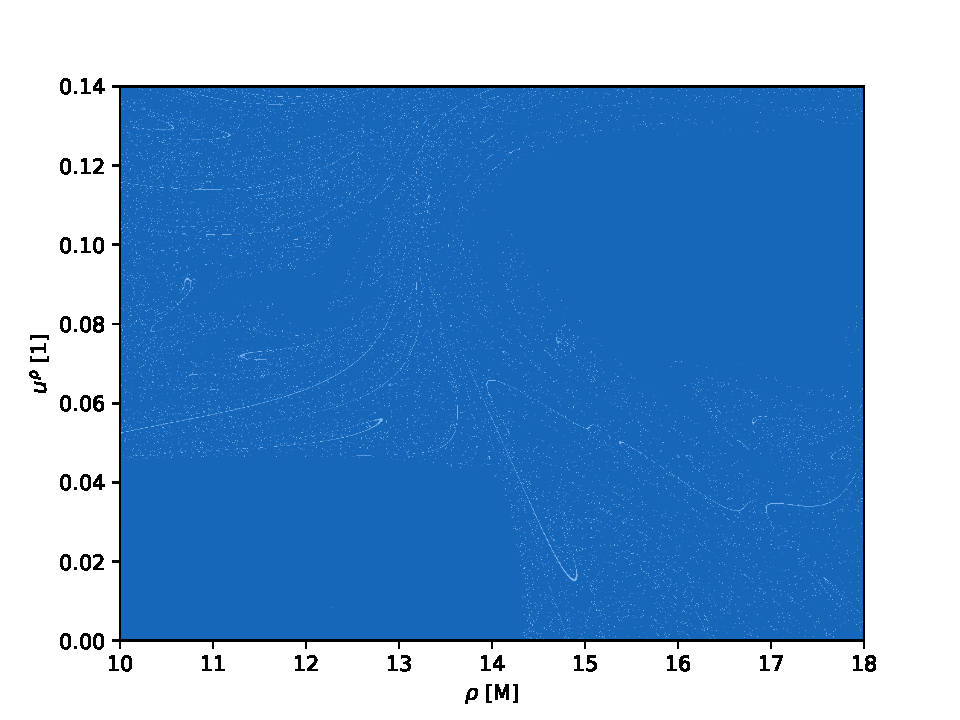
\includegraphics[width=0.82\linewidth]{img/basin_map_sch_bw_1000_1.0_3.943_0.955_20.0_0.5_0.2_0_x86.pdf}
    \caption{Basin map (SCHW+BW) computed on a $1000\times 1000$ grid of initial conditions, $l=3.943M$, $\epsilon=0.955$, $b=20M$, $\mathcal{M}=0.5M$, $z=0.2$ (x86). \basinLegend}
    \label{fig:basin-schw-bw-1000-l3p943-e0p955-b20-M0p5-z0p2-x86}
\end{figure}

\begin{figure}[H]
    \centering
    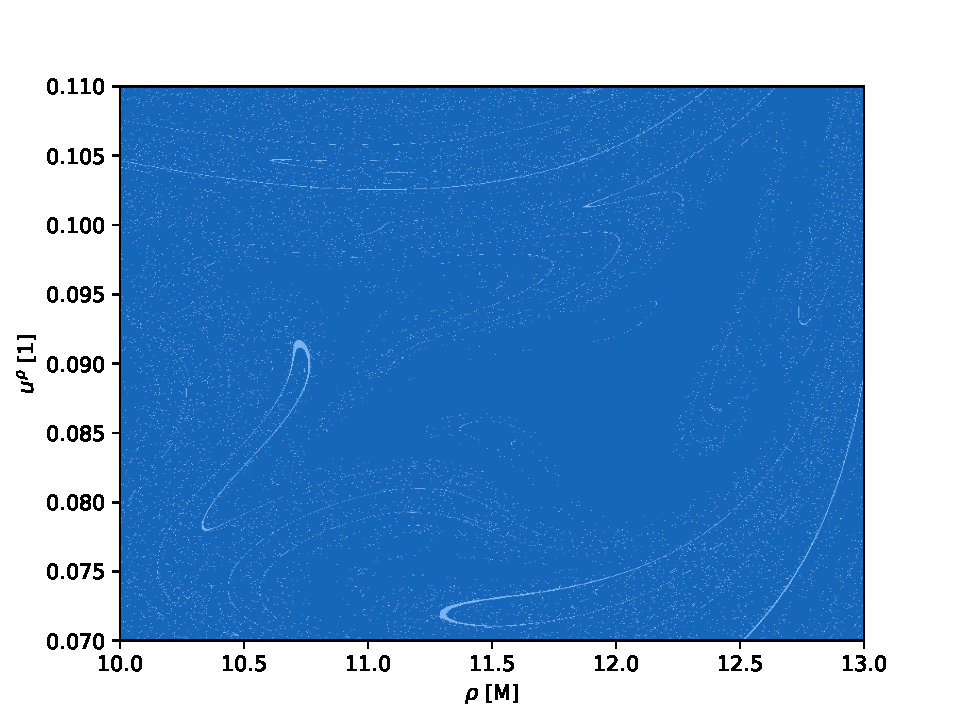
\includegraphics[width=0.82\linewidth]{img/basin_map_sch_bw_700_1.0_3.943_0.955_20.0_0.5_0.2_0_x86.pdf}
    \caption{Basin map (SCHW+BW) computed on a $700\times 700$ grid of initial conditions, $l=3.943M$, $\epsilon=0.955$, $b=20M$, $\mathcal{M}=0.5M$, $z=0.2$ (x86). \basinLegend}
    \label{fig:basin-schw-bw-700-l3p943-e0p955-b20-M0p5-z0p2-x86}
\end{figure}

\begin{figure}[H]
    \centering
    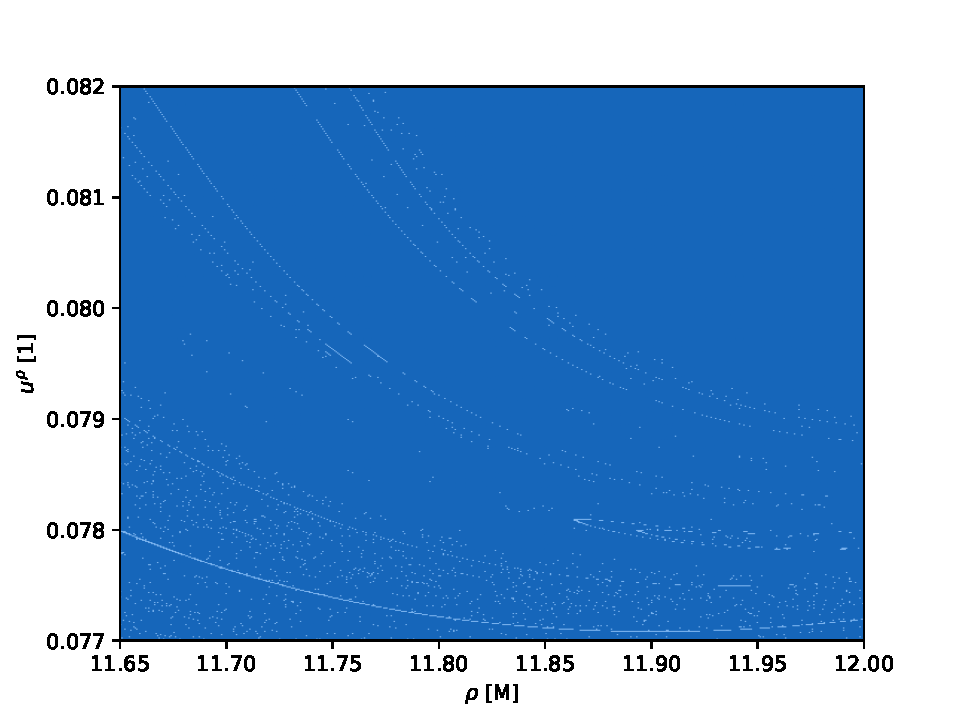
\includegraphics[width=0.82\linewidth]{img/basin_map_sch_bw_500_1.0_3.943_0.955_20.0_0.5_0.2_0_x86.pdf}
    \caption{Basin map (SCHW+BW) computed on a $500\times 500$ grid of initial conditions, $l=3.943M$, $\epsilon=0.955$, $b=20M$, $\mathcal{M}=0.5M$, $z=0.2$ (x86). \basinLegend}
    \label{fig:basin-schw-bw-500-l3p943-e0p955-b20-M0p5-z0p2-x86}
\end{figure}

To compare our results not just visually, but also quantitatively, we shall proceed to calculate the fractal dimension. 

\begin{figure}[H]
    \centering
    \begin{minipage}{0.49\linewidth}
        \centering
        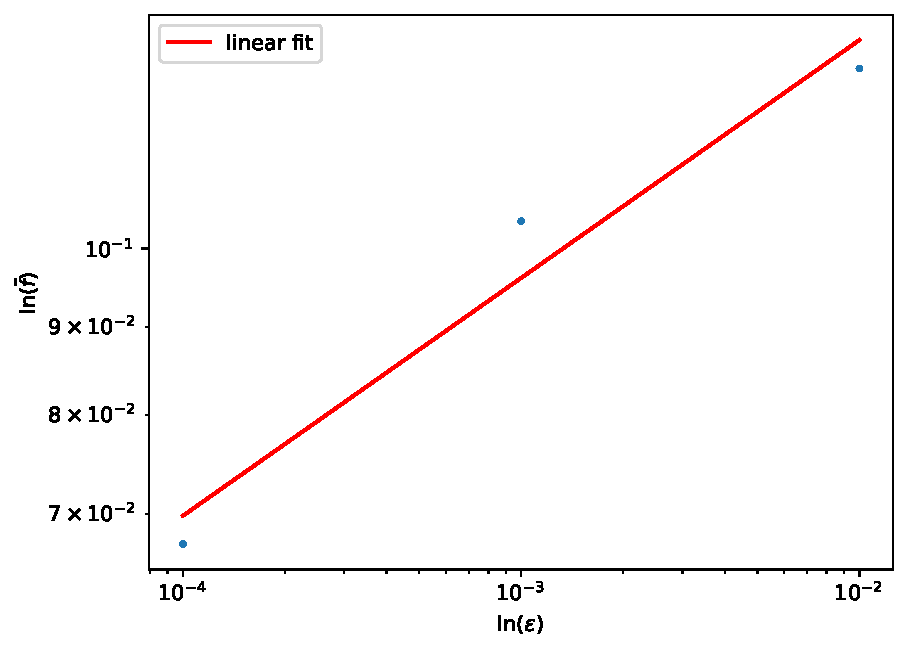
\includegraphics[width=\linewidth]{img/schw_bw_1.0_3.943_0.955_20_0.5_0.2.pdf}
    \end{minipage}\hfill
    \begin{minipage}{0.49\linewidth}
        \centering
        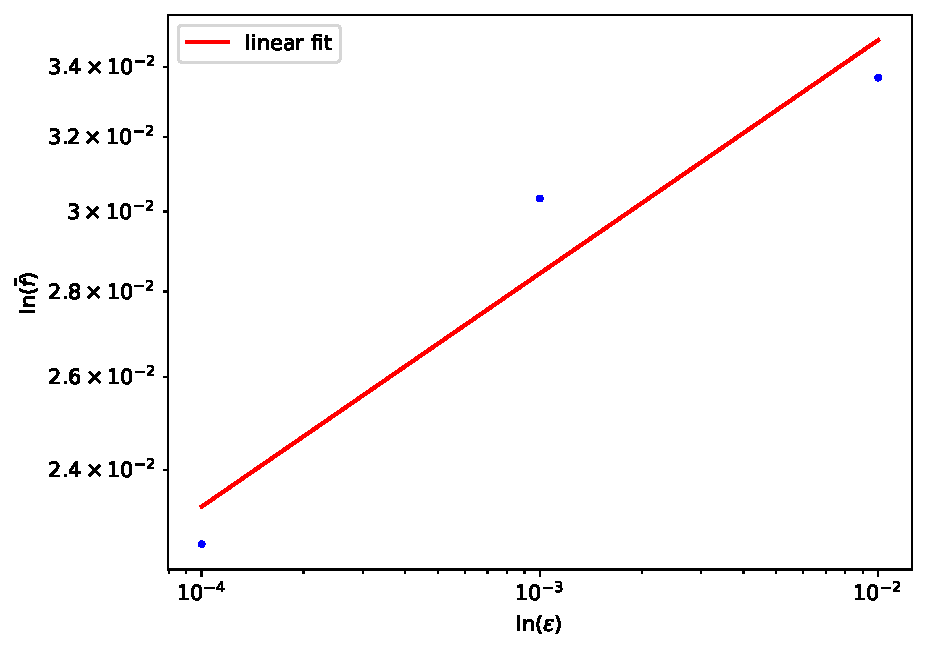
\includegraphics[width=\linewidth]{img/schw_bw_1.0_3.943_0.955_20_0.5_0.2_x86.pdf}
    \end{minipage}
    \caption{Fractal dimension computation (left: ARM; right: x86).}
    \label{fig:fractal-dimension-apple-vs-x86}
\end{figure}

For the basin boundary under the given parameters, we obtained
\begin{equation}
    d_{\mathrm{ARM}} = 1.861 \pm 0.029,
    \qquad
    d_{\mathrm{x86}} = 1.912 \pm 0.024.
    \label{eq:fractal-dimension-arm-x86}
\end{equation}
These values are consistent within their uncertainties, as the corresponding confidence intervals overlap. The high fractal dimension of the basin boundary in both cases, corresponding to the low uncertainty exponent, indicates a high degree of final-state sensitivity to perturbations of the initial conditions. However, these values are not consistent with the values from Sychrovsky~\cite{Sychrovsky2020}. The discussion above for the visual inconsistency applies here as well.

Another interesting effect that is caused by precision is the web-like numerical artifact. 

\begin{figure}[H]
    \centering
    \begin{minipage}{0.48\linewidth}
        \centering
        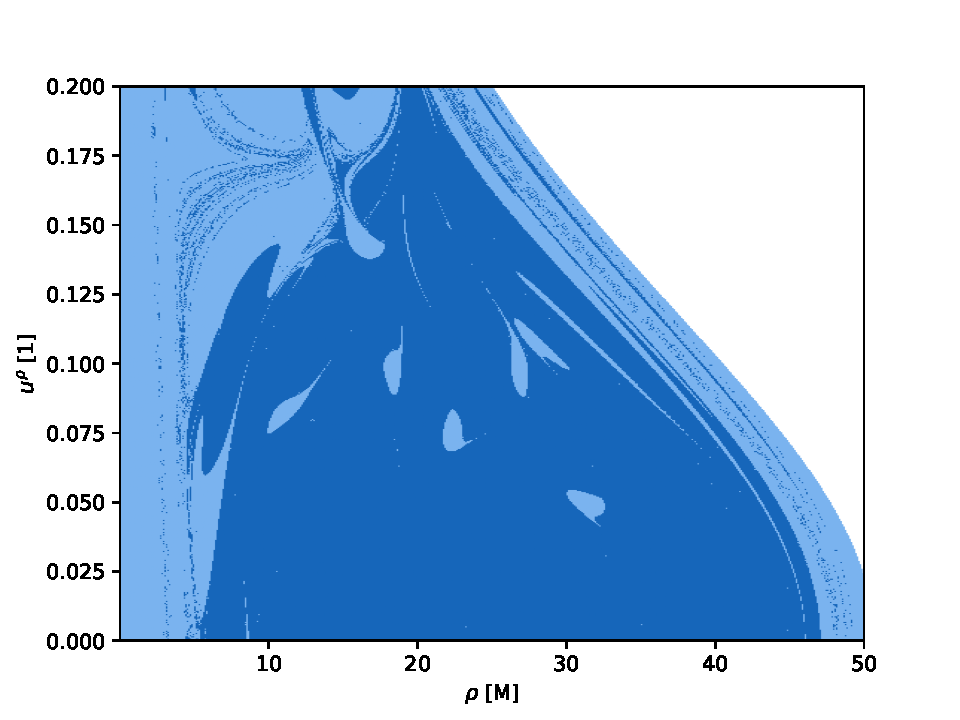
\includegraphics[width=\linewidth]{img/basin_map_sch_bw_500_1.0_3.75_0.977_20.0_0.3_0.0_0_x86.pdf}
    \end{minipage}\hfill
    \begin{minipage}{0.48\linewidth}
        \centering
        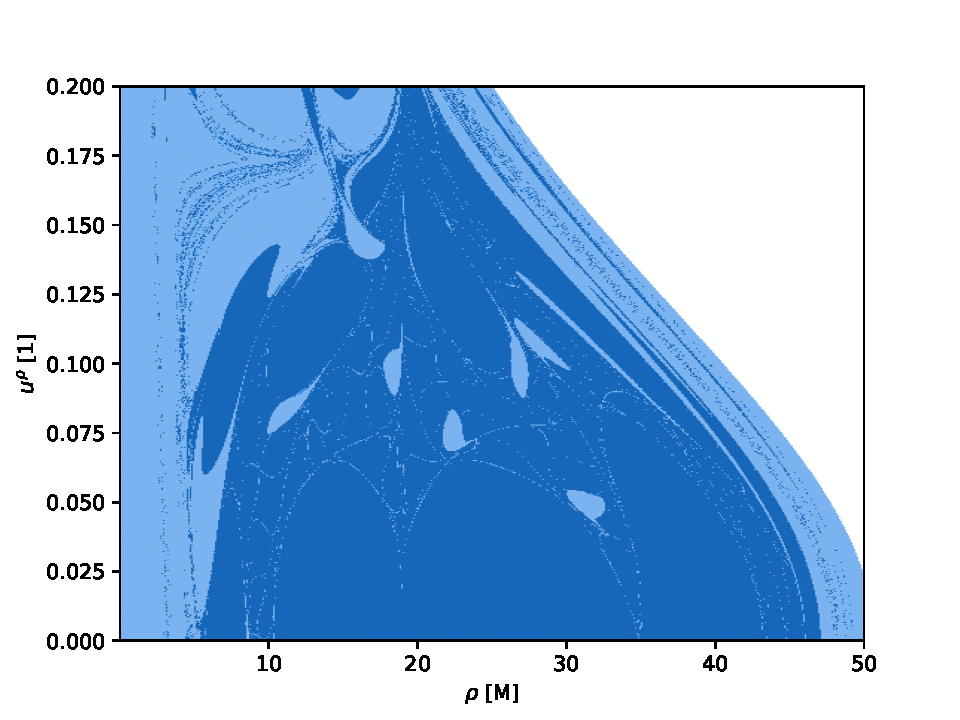
\includegraphics[width=\linewidth]{img/basin_map_sch_bw_500_1.0_3.75_0.977_20.0_0.3_0.0_0.pdf}
    \end{minipage}
    \caption{Basin map comparison (left: x86; right: ARM); computed on a $500\times 500$ grid of initial conditions, $l=3.75M$, $\epsilon=0.977$, $b=20M$, $z=0.0$. \basinLegend}
    \label{fig:basin-x86-arm-03}
\end{figure}

\begin{figure}[H]
    \centering
    \begin{minipage}{0.48\linewidth}
        \centering
        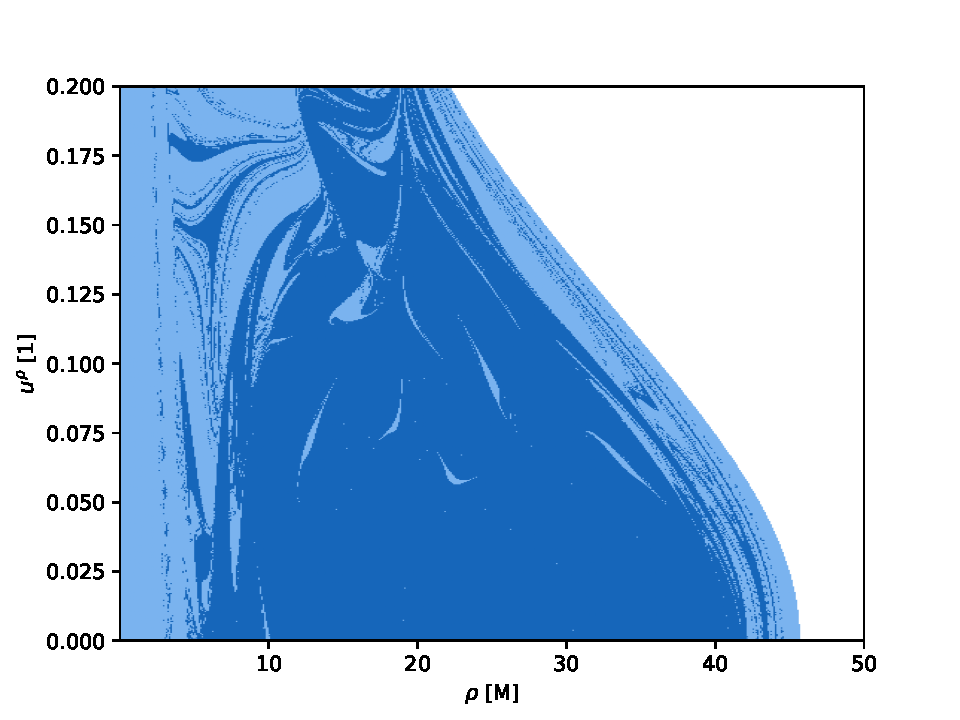
\includegraphics[width=\linewidth]{img/basin_map_sch_bw_500_1.0_3.75_0.977_20.0_0.2_0.0_0_x86.pdf}
    \end{minipage}\hfill
    \begin{minipage}{0.48\linewidth}
        \centering
        
\includegraphics[width=\linewidth]{img/basin_map_sch_bw_500_1.0_3.75_0.977_20.0_0.2_0.0_0.pdf}
    \end{minipage}
    \caption{Basin map comparison (left: x86; right: ARM); computed on a $500\times 500$ grid of initial conditions, $l=3.75M$, $\epsilon=0.977$, $b=20M$, $z=0.0$. \basinLegend}
    \label{fig:basin-x86-arm-02}
\end{figure}

\begin{figure}[H]
    \centering
    \begin{minipage}{0.48\linewidth}
        \centering
        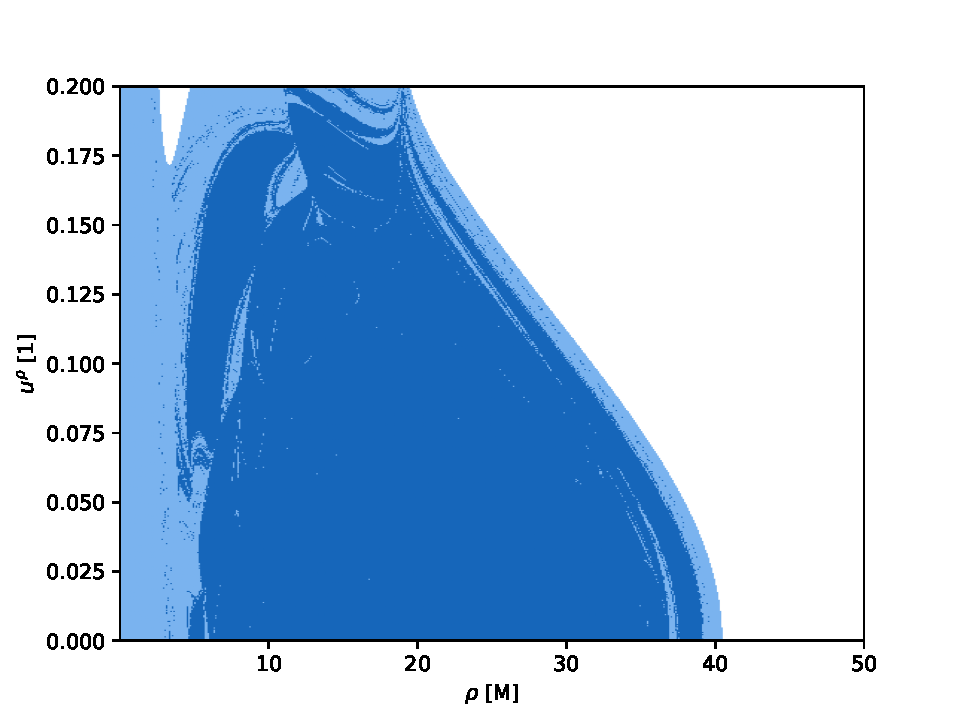
\includegraphics[width=\linewidth]{img/basin_map_sch_bw_500_1.0_3.75_0.977_20.0_0.1_0.0_0_x86.pdf}
    \end{minipage}\hfill
    \begin{minipage}{0.48\linewidth}
        \centering
        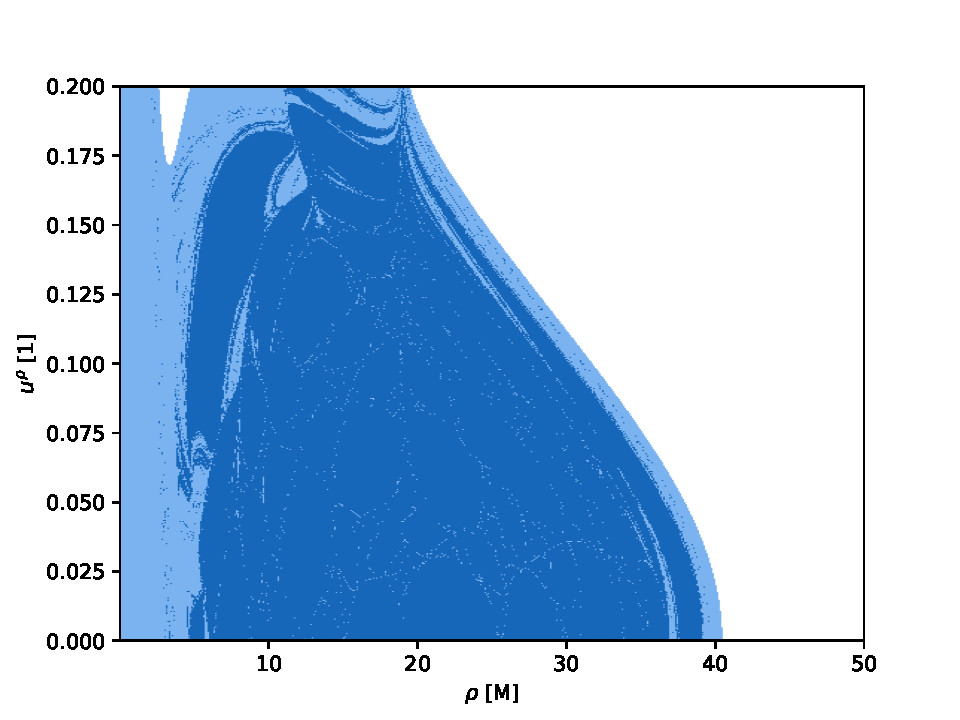
\includegraphics[width=\linewidth]{img/basin_map_sch_bw_500_1.0_3.75_0.977_20.0_0.1_0.0_0.pdf}
    \end{minipage}
    \caption{Basin map comparison (left: x86; right: ARM); computed on a $500\times 500$ grid of initial conditions, $l=3.75M$, $\epsilon=0.977$, $b=20M$, $z=0.0$. \basinLegend}
    \label{fig:basin-x86-arm-01}
\end{figure}

\subsection{Comparison with Poincar\'e sections}

As a second validation of the Schwarzschild black-hole plus Bach--Weyl
ring implementation, we compare our basin maps with the equatorial
Poincar\'e sections shown by Polcar, Sukova and Semerak~\cite{Polcar2019}.
Their sections were computed for geodesics with
\(\ell=3.75M\), \(\epsilon=0.977\), and ring radius \(b=20M\), while
the relative ring mass \(\mathcal{M}/M\) was varied. The reference
Poincar\'e sections are reproduced in Figure~\ref{fig:poincare-schw-bw-chaos-v}.

\begin{figure}[H]
    \centering
    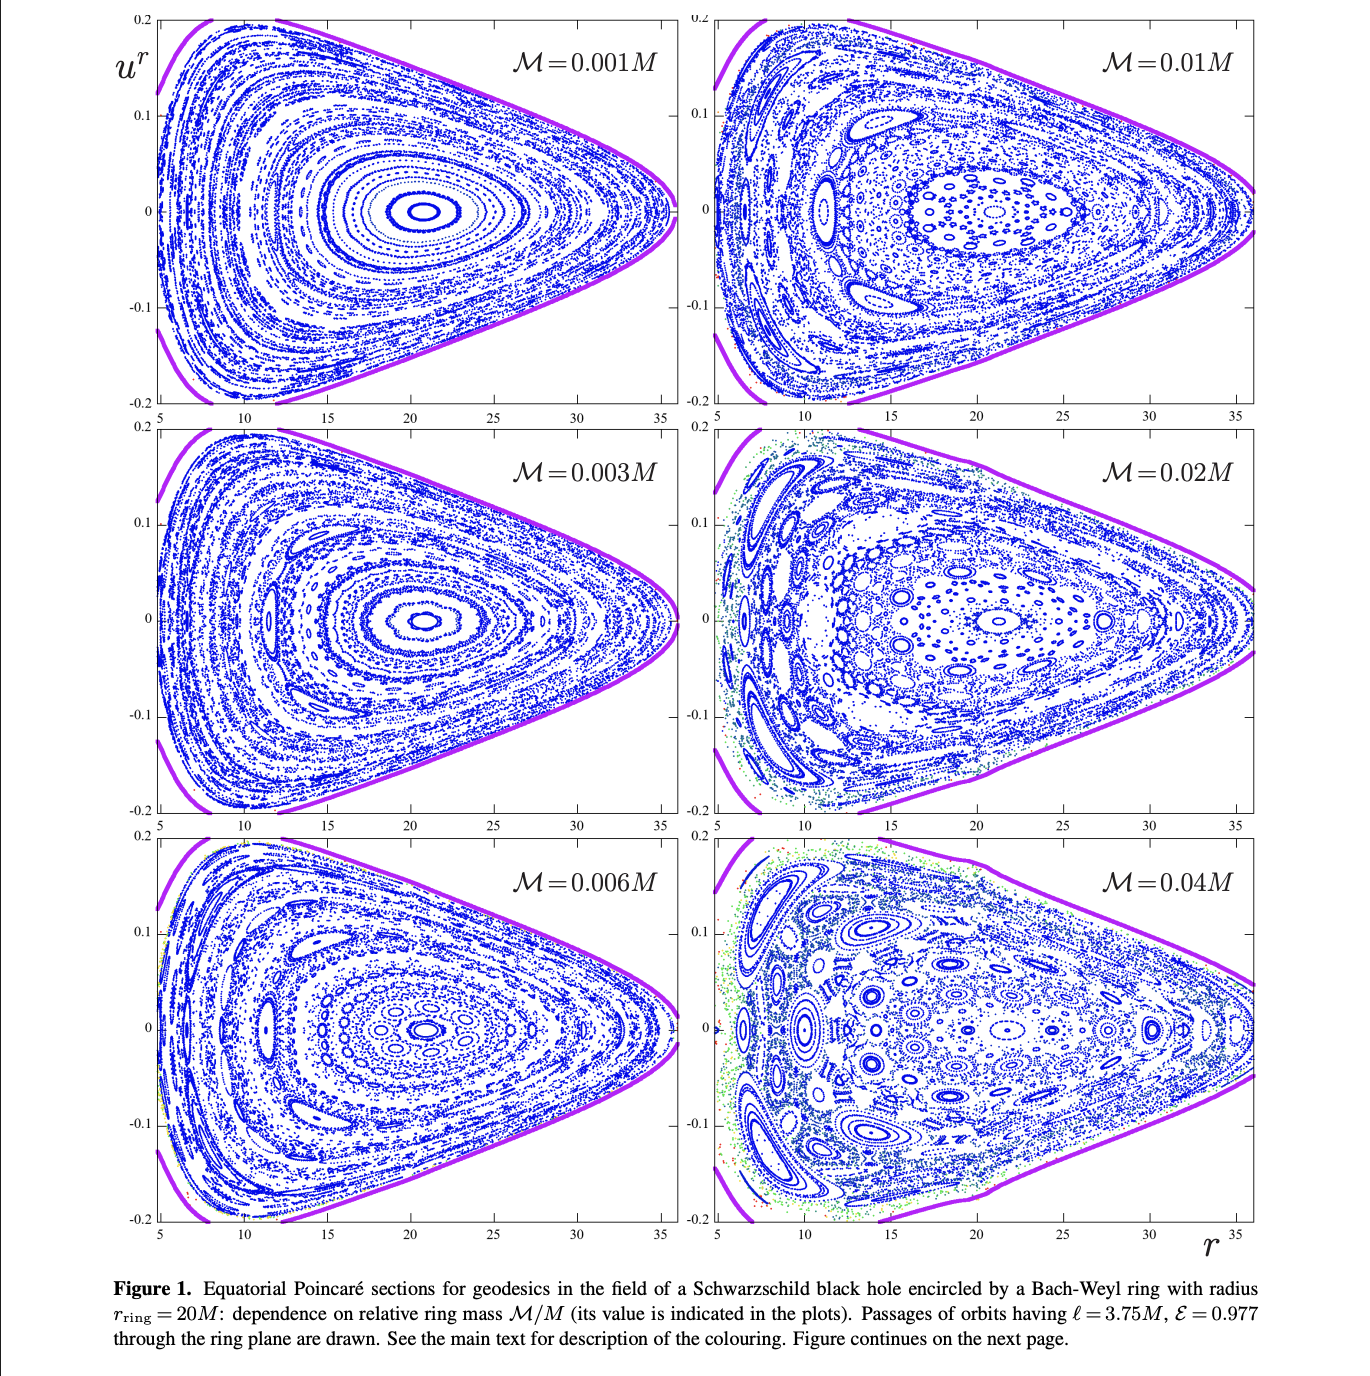
\includegraphics[width=0.95\linewidth]{img/poincare_sections_schw_bw_chaos_V.png}
    \caption{Reference equatorial Poincar\'e sections for the
    Schwarzschild black hole with a Bach--Weyl ring, with
    \(b=20M\), \(\ell=3.75M\), and \(\epsilon=0.977\). The values of
    \(\mathcal{M}/M\) are indicated in the individual panels.}
    \label{fig:poincare-schw-bw-chaos-v}
\end{figure}

For the comparison we use only the x86 calculations, since these were
computed with extended precision \texttt{long double}. The basin maps in
Figure~\ref{fig:basin-schw-bw-chaos-v-x86} use the same values of
\(\ell\), \(\epsilon\), \(b\), and the equatorial plane \(z=0\). The
ring-mass values are those available in our x86 result set, so this is a
comparison of the trend with increasing perturbation, not a
panel-by-panel reproduction of the exact masses in
Figure~\ref{fig:poincare-schw-bw-chaos-v}. They are also not Poincar\'e
sections: each pixel represents an initial condition in the
\((\rho_0,u^\rho_0)\) plane and is classified according to the final
outcome of the numerical integration. In addition, the reference sections
use Schwarzschild \(r\), while our basin maps are plotted in Weyl
\(\rho\). Nevertheless, the comparison is useful because both diagnostics
probe the equatorial reduced phase space and both react visibly to the
increasing Bach--Weyl perturbation.

\begin{figure}[H]
    \centering
    \begin{minipage}{0.32\linewidth}
        \centering
        \small \(\mathcal{M}=0.07M\)
        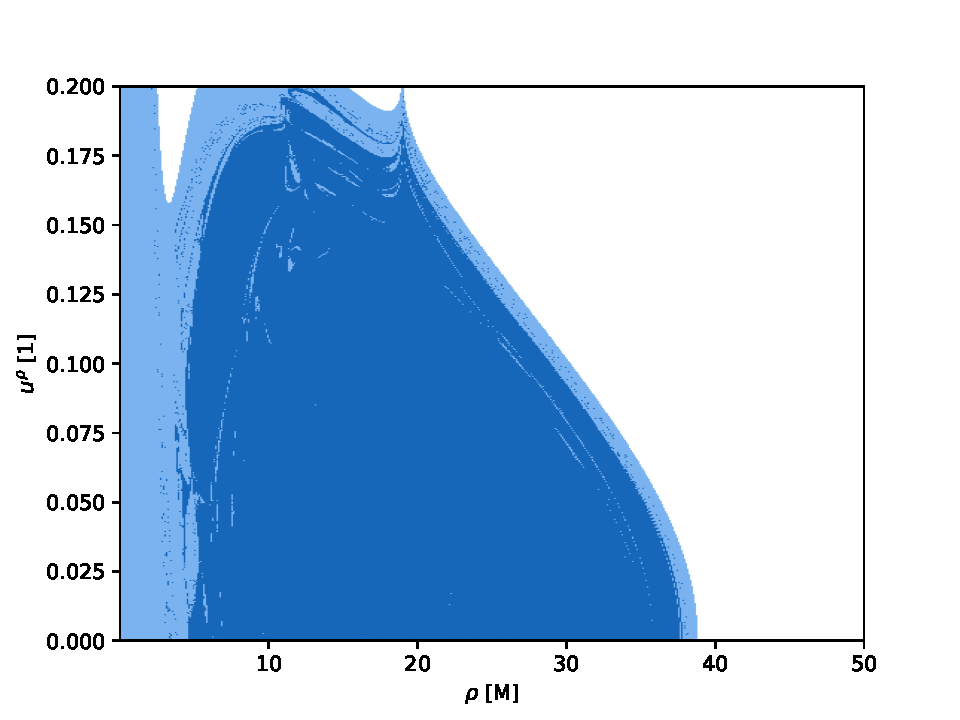
\includegraphics[width=\linewidth]{img/basin_map_sch_bw_500_1.0_3.75_0.977_20.0_0.07_0.0_0_x86.pdf}
    \end{minipage}\hfill
    \begin{minipage}{0.32\linewidth}
        \centering
        \small \(\mathcal{M}=0.1M\)
        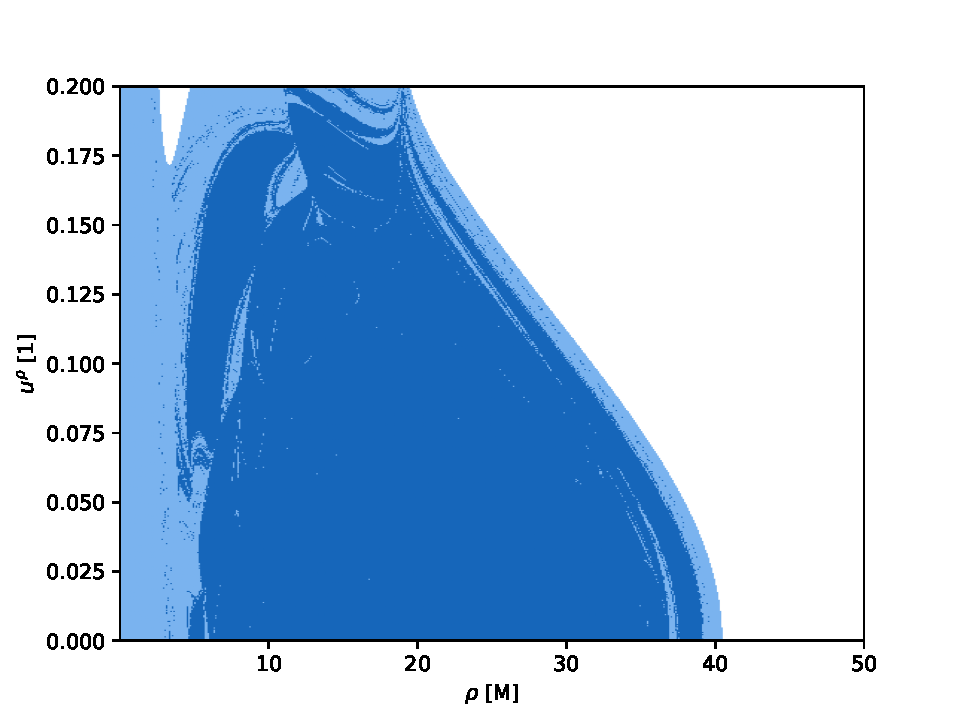
\includegraphics[width=\linewidth]{img/basin_map_sch_bw_500_1.0_3.75_0.977_20.0_0.1_0.0_0_x86.pdf}
    \end{minipage}\hfill
    \begin{minipage}{0.32\linewidth}
        \centering
        \small \(\mathcal{M}=0.2M\)
        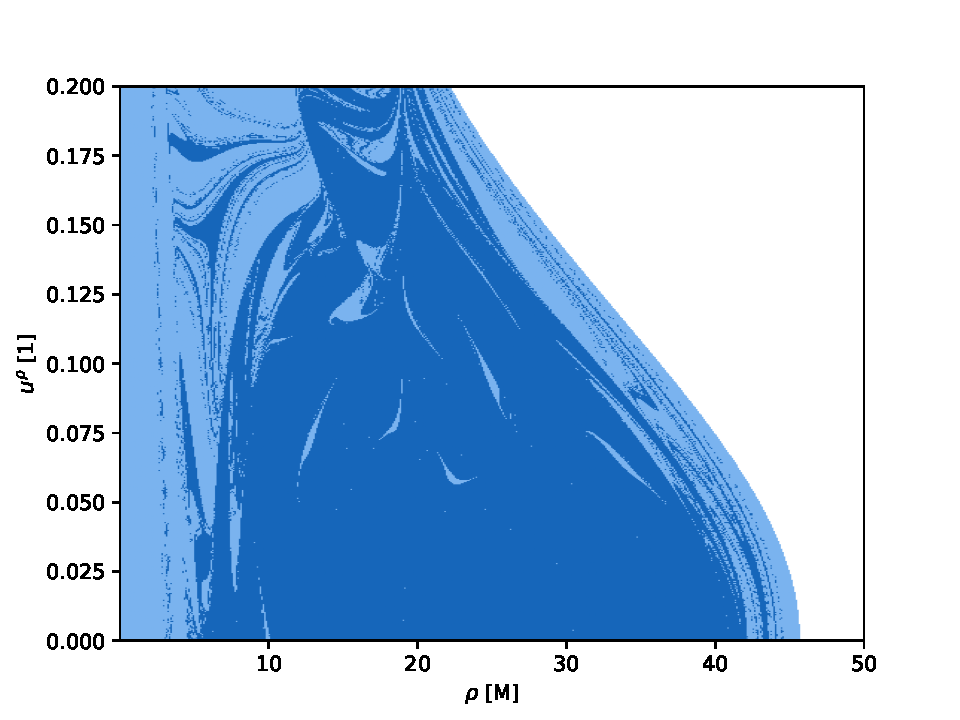
\includegraphics[width=\linewidth]{img/basin_map_sch_bw_500_1.0_3.75_0.977_20.0_0.2_0.0_0_x86.pdf}
    \end{minipage}

    \vspace{0.6em}

    \begin{minipage}{0.32\linewidth}
        \centering
        \small \(\mathcal{M}=0.3M\)
        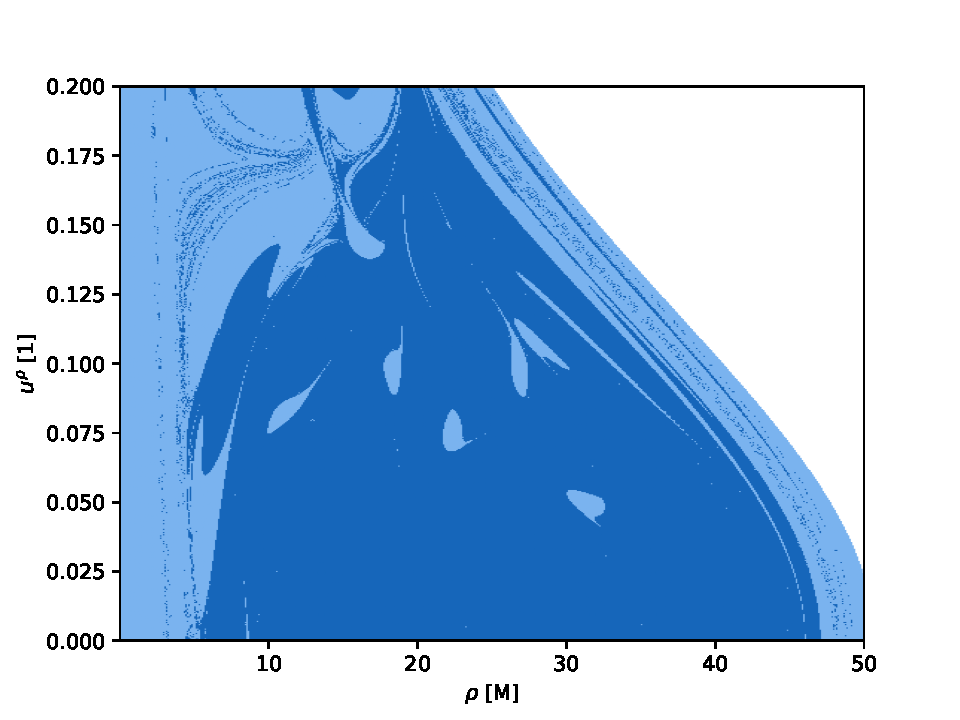
\includegraphics[width=\linewidth]{img/basin_map_sch_bw_500_1.0_3.75_0.977_20.0_0.3_0.0_0_x86.pdf}
    \end{minipage}\hfill
    \begin{minipage}{0.32\linewidth}
        \centering
        \small \(\mathcal{M}=0.6M\)
        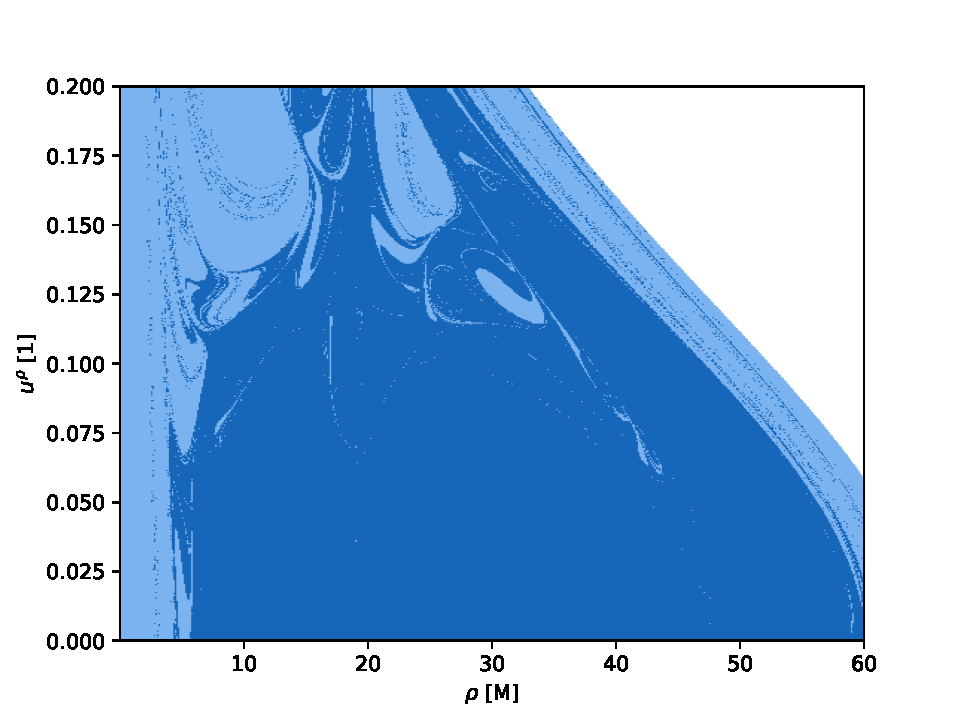
\includegraphics[width=\linewidth]{img/basin_map_sch_bw_500_1.0_3.75_0.977_20.0_0.6_0.0_0_x86.pdf}
    \end{minipage}\hfill
    \begin{minipage}{0.32\linewidth}
        \centering
        \small \(\mathcal{M}=1.1M\)
        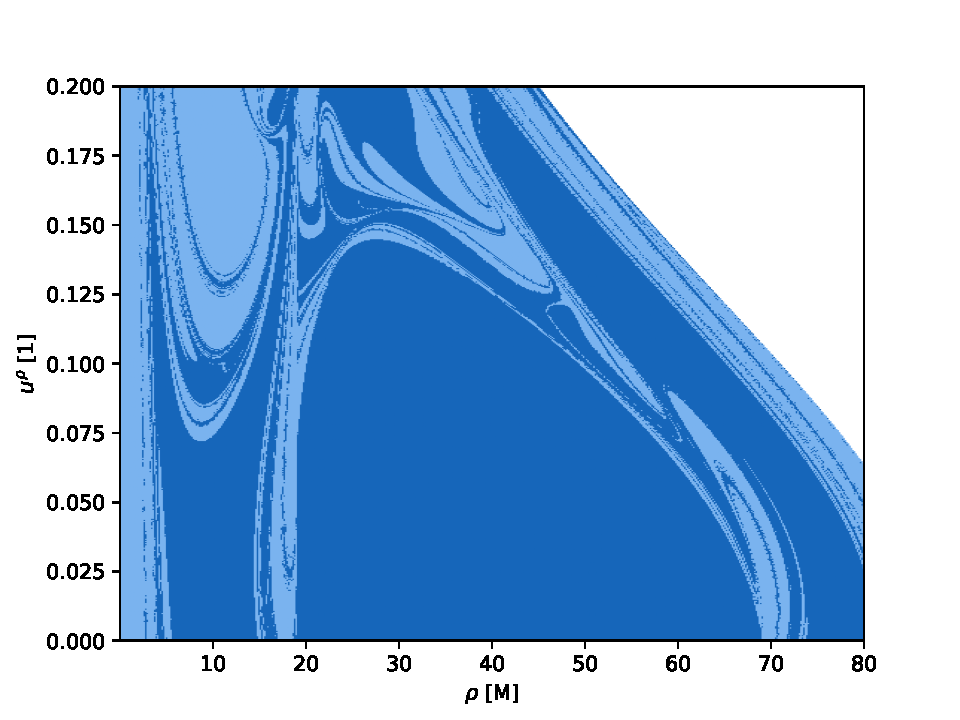
\includegraphics[width=\linewidth]{img/basin_map_sch_bw_500_1.0_3.75_0.977_20.0_1.1_0.0_0_x86.pdf}
    \end{minipage}
    \caption{Basin maps (SCHW+BW) computed on a \(500\times500\) grid
    of initial conditions for \(l=3.75M\), \(\epsilon=0.977\),
    \(b=20M\), \(z=0\), and increasing ring mass \(\mathcal{M}\) (x86).
    \basinLegend}
    \label{fig:basin-schw-bw-chaos-v-x86}
\end{figure}

The comparison is necessarily qualitative. A Poincar\'e section separates
regular invariant curves, resonant islands and stochastic layers inside
the bounded part of phase space, whereas the basin map records whether a
chosen initial condition survives until \(T_{\mathrm{MAX}}\) or reaches
the singular part of the space-time earlier. Therefore one should not
expect a one-to-one correspondence between individual islands in
Figure~\ref{fig:poincare-schw-bw-chaos-v} and coloured domains in
Figure~\ref{fig:basin-schw-bw-chaos-v-x86}. The relevant point is the
common trend. In the reference sections, increasing \(\mathcal{M}\)
destroys the simple near-integrable structure: invariant curves are
gradually replaced by resonant island chains and broader chaotic layers.
In our x86 basin maps the same increase of the perturbing ring mass
produces a progressively more complicated basin boundary, especially
near the edge of the accessible region and near the ring. This supports
the interpretation that the final-state sensitivity visible in the basin
maps is associated with the same loss of regularity that is seen directly
in the Poincar\'e sections.
